\documentclass{article}
\usepackage{graphicx} % Required for inserting images
\usepackage{listings}
\usepackage{xcolor}
\definecolor{jsonpurple}{RGB}{128,0,128}
\definecolor{jsonblue}{RGB}{0,0,255}

\lstdefinelanguage{json}{
    basicstyle=\small\ttfamily,
    showstringspaces=false,
    breaklines=true,
    frame=lines,
    backgroundcolor=\color{white},
    string=[s]{"}{"},
    stringstyle=\color{jsonpurple},
    comment=[l]{//},
    commentstyle=\color{gray}\ttfamily,
    keywordstyle=\color{jsonblue},
    morekeywords={true,false,null},
    keywords=[2]{},
    keywordstyle=[2]\color{jsonblue},
    identifierstyle=\color{black},
}

\lstset{
    language=Python,
    basicstyle=\ttfamily,
    keywordstyle=\color{blue},
    commentstyle=\color{gray},
    stringstyle=\color{green},
    numbers=left,
    numberstyle=\tiny,
    numbersep=5pt,
    breaklines=true,
    breakatwhitespace=true,
    frame=single,
    showstringspaces=false,
    captionpos=b,
    tabsize=4
}

\title{Simple Blockchain Implementation}
\author{Jan Chlebek
\and Szymon Krysztopolski
}
\date{June 2023}

\begin{document}

\maketitle

The objective of this project is to implement a basic blockchain structure that can be used to
store and verify transactions. The blockchain should include the necessary components such as blocks,
transactions, and cryptographic mechanisms to ensure data integrity and security.

\section{Selected development tools}
Our blockchain was implemented using Python 3.10.
As a base of cryptography in the project we decided to use cryptography and hashlib library combination


\section{Overall algorithm implementation and adpoted simplifications}
When planning the implementation, we decided not to proceed with any distributed form of computing. Our blockchain is stored as nodes on centralised single-process instance of server orchestrated by System user.

\begin{enumerate}
  \item Blockchain is a one-way list. The entire run is controlled by the System (less problem with parallelism).
  \item Users are known in advance and have their asymmetric key pair, login and password (stored as hash). There is no mechanism for adding them (I will focus on blockchain). They are hardcoded in the appropriate dictionary initialized at program startup.
  \item The blocks are stored in text files and created by System user. The file has the following characteristics:
    \begin{itemize}
        \item the file name is a hash (we assume unique)
        \item each block / block file has a JSON with the following content:
        \begin{itemize}
            \item subtitle TITLE encrypted with the author's private key
            \item transactions added by the author of the block on behalf of the user who generated the transactions
            \item hash of the previous block
        \item The first block is named INIT and is generated by the System user.
	    \item The last block in the chain has no value indicating the previous block. When a block is added, this information is completed.
        \item When blockchain system is restarted, all existing blocks signatures are checked for validity to ensure the system has not been compromised.
        \end{itemize}
    \end{itemize}
    \item Each user can add a new set of new transactions. Request accepts the System. It then sends a TASK to all users. The first one to execute it gets the opportunity to add a block.
    \item We are working based on Proof-of-Work TASK which requires the generation of a hash starting with zero
\end{enumerate}


\section{Code snippets}

\subsection{Block file structure}
filename: SHA256 hash
\begin{lstlisting}[language=json]
{
    "block_name": "SHA256 hash",
    "timestamp": "Encrypted message using RSA with OAEP padding",
    "transactions": [
        "List of transactions: USER: ------ Object",
        "AliceWonder: ------ Haste makes waste."
    ],
    "signer": "Username of signer",
    "signature": "RSA signature with PSS padding",
    "prev_block": "SHA256 hash of previous block"
}
\end{lstlisting}

\subsection{Proof-of-work}
\begin{lstlisting}[language=json]
    def manager.is_winner(hash: str) -> bool:
        return hash.startswith("0")

    active_challange = True
    while active_challange:
        for i in challenge_order:
            user = User_list[i]
            if manager.is_winner(user.get_base64_hash()):
                manager.add_block_to_blockchain(user, new_transactions)
                active_challange = False
                break
\end{lstlisting}

\section{How to use the program}

Our blockchain program logs into System user account when started. The startup panel has several options available. 

\vspace{0.5cm}
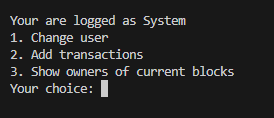
\includegraphics{start.png}

\begin{itemize}
    \item 1. User's account change - this option allows to change current account after provide proper credentials (e.g. JohnDoe, qwerty123). 
    \item 2. Add transaction. A logged-in user can add new transactions. In current version of the program, this option allows you to specify how many predefined transactions are to be added to the blockchain. The maximum value is 5. Transactions are randomly selected from specific sample table.
    \item 3. Displays the current blocks with owners. In this option, the owner is the account that added block to the blockchain.
    
    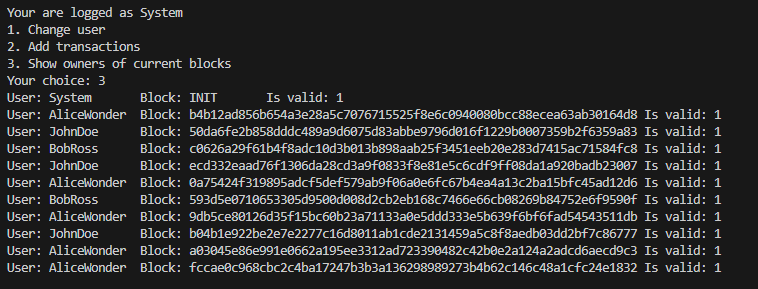
\includegraphics[width=\textwidth]{block_list.png}
    \item e. Exits program.
\end{itemize}

If the program is run with \textbf{{-}{-}init} as a parameter, the program will remove all blocks.

If the program is run with \textbf{{-}{-}test xxx} as a parameter (where xxx is a number), the program will remove all blocks and create xxx number of 5 transaction blocks as a benchmark.

\end{document}


